\documentclass[12pt, twoside]{article}
\usepackage[letterpaper, margin=1in, headsep=0.5in]{geometry}
\usepackage[english]{babel}
\usepackage[utf8]{inputenc}
\usepackage{amsmath}
\usepackage{amsfonts}
\usepackage{amssymb}
\usepackage{tikz}
\usetikzlibrary{quotes, angles}
\usepackage{graphicx}
\usepackage{enumitem}
\usepackage{multicol}

\newif\ifmeta
\metatrue %print standards and topics tags

\title{Regents Geometry}
\author{Chris Huson}
\date{September 2020}

\usepackage{fancyhdr}
\pagestyle{fancy}
\fancyhf{}
\renewcommand{\headrulewidth}{0pt} % disable the underline of the header
\raggedbottom


\fancyhead[LE]{\thepage}
\fancyhead[RO]{\thepage \\ Name: \hspace{4cm} \,\\}
\fancyhead[LO]{BECA / Dr. Huson / Geometry 09-Congruence-transformations\\* pset ID: 158}

\begin{document}

\subsubsection*{9-4bDN-reflection}
\begin{enumerate}
\item Which of the following would map $\triangle CAT \rightarrow \triangle C'A'T'$?  \vspace{0.5cm}
    \begin{multicols}{2}
      \begin{itemize}
        \item[T \quad F \quad] Reflected across the $y$-axis
        \item[T \quad F \quad] Translated six to the left, down zero
        \item[T \quad F \quad] Reflected across the $y$-axis, then slid to the left two
        \item[T \quad F \quad] $(x,y) \rightarrow (x-6, y+0)$
        \item[T \quad F \quad] Rotated $90^\circ$ counterclockwise around the origin
        \item[T \quad F \quad] Reflected across the line $x=-1$
      \end{itemize}
      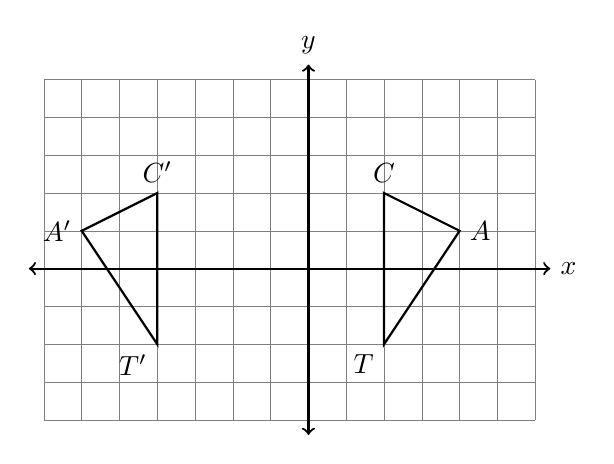
\begin{tikzpicture}[scale=.48]
        \draw [help lines] (-7,-4) grid (6,5);
        \draw [thick, <->] (-7.4,0) -- (6.4,0) node [right] {$x$};
        \draw [thick, <->] (0,-4.4)--(0,5.4) node [above] {$y$};  
        \draw [thick]
        (2,2) node[above] {$C$}--
        (4,1) node[right] {$A$}--
        (2,-2) node[below left] {$T$}--cycle;
        \draw [thick]
        (-4,2) node[above] {$C'$}--
        (-6,1) node[left] {$A'$}--
        (-4,-2) node[below left] {$T'$}--cycle;
      \end{tikzpicture}
    \end{multicols}

\item Draw the line of reflection used to map $\triangle ABC$ onto $\triangle A'B'C'$.
  \begin{center}
      \begin{tikzpicture}%[scale=.48]
      %\draw [help lines] (-7,-2) grid (7,6);
      %\draw [thick, <->] (-7.4,0) -- (7.4,0) node [right] {$x$};
      %\draw [thick, <->] (0,-2.4)--(0,6.4) node [above] {$y$};  
      \draw [thick]
        (1,5) node[above] {$A$}--
        (3,4) node[above ] {$B$}--
        (-1,2) node[below left] {$C$}--cycle;
      \draw [thick]
      (5,1) node[right] {$A'$}--
      (4,3) node[above right] {$B'$}--
      (2,-1) node[below right] {$C'$}--cycle;
    \end{tikzpicture}
  \end{center}

\item Draw the line of reflection for each diagram below. \\
    \begin{tikzpicture}[scale=.48]
      %\draw [help lines] (-10,-7) grid (10,7);
      \draw [thick, <->] (-4.4,0) -- (8.4,0) node [right] {$x$};
      \draw [thick, <->] (0,-2.4)--(0,7.4) node [above] {$y$};  
      \draw [thick](5,1)--(7,2)--(8,5)--(6,5)--cycle;  
      \draw [thick](-1,1)--(-3,2)--(-4,5)--(-2,5)--cycle;
    \end{tikzpicture} \hspace{1.7cm}
    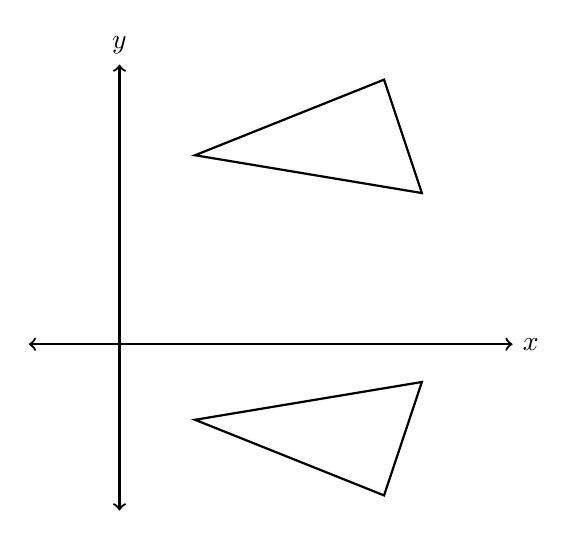
\begin{tikzpicture}[scale=.48]
      %\draw [help lines] (-10,-7) grid (10,7);
      \draw [thick, <->] (-2.4,0) -- (10.4,0) node [right] {$x$};
      \draw [thick, <->] (0,-4.4)--(0,7.4) node [above] {$y$};  
      \draw [thick](2,5)--(7,7)--(8,4)--cycle;  
      \draw [thick](2,-2)--(7,-4)--(8,-1)--cycle;
    \end{tikzpicture}

\newpage
\item Determine and state the sequence of transfromations applied to map $BECA$ to $B'E'C'A'$ and then to $B''E''C''A''$.
  \begin{center}
      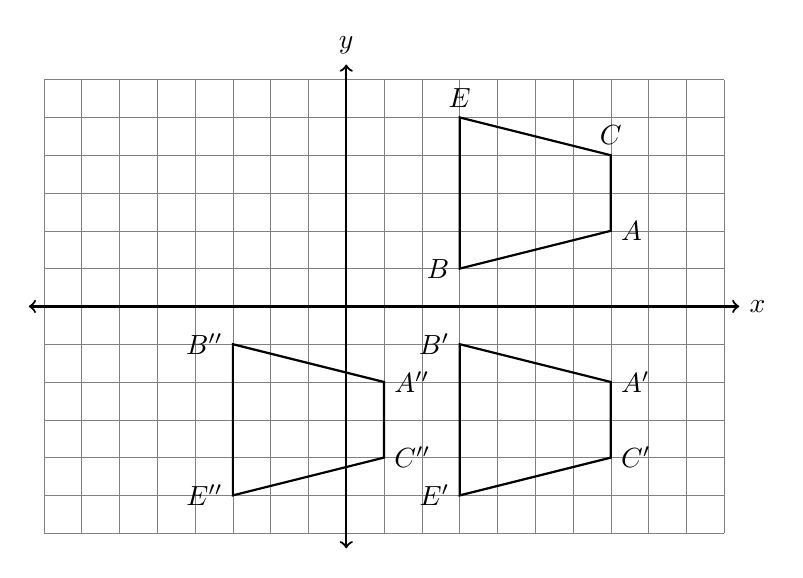
\begin{tikzpicture}[scale=.48]
      \draw [help lines] (-8,-6) grid (10,6);
      \draw [thick, <->] (-8.4,0) -- (10.4,0) node [right] {$x$};
      \draw [thick, <->] (0,-6.4)--(0,6.4) node [above] {$y$};  
      \draw [thick]
        (3,1) node[left] {$B$}--
        (3,5) node[above] {$E$}--
        (7,4) node[above] {$C$}--
        (7,2) node[right] {$A$}--cycle;
      \draw [thick]
        (3,-1) node[left] {$B'$}--
        (3,-5) node[left] {$E'$}--
        (7,-4) node[right] {$C'$}--
        (7,-2) node[right] {$A'$}--cycle; 
      \draw [thick]
        (-3,-1) node[left] {$B''$}--
        (-3,-5) node[left] {$E''$}--
        (1,-4) node[right] {$C''$}--
        (1,-2) node[right] {$A''$}--cycle; 
    \end{tikzpicture}
  \end{center}

\end{enumerate}
\end{document}